%====================================================
%
% Author: Dipl.-Inf. Xavier NOUMBISSI NOUNDOU, Ph.D. (A.B.D.)
% Email:  xnoundou7@gmail.com
%
%====================================================
\documentclass[12pt, a4paper]{article}
\NeedsTeXFormat{LaTeX2e}

%---------------------------- PACKAGE INCLUSION -------------------------------
% This group renders characters clearer and more precise

\RequirePackage[bitstream-charter,cal,expert]{mathdesign}
\RequirePackage{latexsym}

\usepackage{geometry}
\geometry{a4paper,
		  %showframe=true,
		  %margin=2.75em,
		  %a4paper,
		  %total={170mm,257mm},
		  top=3.5em,
		  left=3em,
		  right=3em,
		  bottom=3.39em
		  }

\usepackage[default]{cantarell}
\usepackage{graphicx}
\usepackage{xspace}
\usepackage[parfill]{parskip} % Activate to begin paragraphs with an empty line rather than an indent
\usepackage{paralist} % very flexible & customisable lists (eg. enumerate/itemize, etc.)
\usepackage{listings} % for lstset definitions
\usepackage{url}
\usepackage{subfig} % make it possible to include more than one captioned figure/table in a single float
\usepackage{epsfig}
\usepackage{booktabs}
%\usepackage{enumitem} %funny itemize icons
\usepackage{verbatim}
\usepackage{tcolorbox}

\usepackage{pagecolor}

\usepackage{amsmath}
\newcommand{\mathbold}[1]{\text{\textbf{#1}}}

\usepackage{xcolor}
\definecolor{yerothColorOrange}{RGB}{242, 161, 0}   
\definecolor{yerothColorBlue}{RGB}{77 , 93 , 254}
\definecolor{yerothColorRed}{RGB}{254, 48 , 48}
\definecolor{yerothColorGray}{RGB}{198, 198, 198}
\definecolor{yerothColorDarkgray}{RGB}{60, 60 , 60}
\definecolor{yerothColorIndigo}{RGB}{83, 0, 125}
\definecolor{yerothColorGreen}{RGB}{2  , 160, 70}
\definecolor{forestgreen}{RGB}{2,160,70}    
\definecolor{mediumblue}{RGB}{7,43,205}    
\definecolor{firebrickred}{RGB}{178,34,34}
\definecolor{listingray}{gray}{0.9}
\definecolor{lbcolor}{rgb}{0.9,0.9,0.9}
\definecolor{darkgreen}{rgb}{0,0.35,0}
\definecolor{medgreen}{rgb}{0,0.5,0}
\definecolor{lightgreen}{rgb}{0.5,0.7,0.5}
\definecolor{pmcolour}{rgb}{0.5,0.7,0.5}
\definecolor{medgrey}{rgb}{0.6,0.6,0.6}
\definecolor{purplish}{rgb}{0.4,0,0.6}
\definecolor{brightred}{rgb}{1,0.2,0.2}

\newcommand{\diplinfn}{Dipl.--Inf.\xspace}

\newcommand{\yerenlabs}{\textsc{YEROTH~R\&D}\xspace}

\newcommand{\yerotherp}{\textcolor{yerothColorBlue}{\sc YEROTH--ERP--$3.0$}\xspace}

\newcommand{\saperp}{SAP Business One\xspace}

\newcommand{\sageerp}{Sage Gescom i$7$\xspace}

\newcommand{\myfullacademicname}{Xavier NOUMBISSI NOUNDOU,~Dipl.--Inf.,~Ph.D.~(ABD)\xspace}

\usepackage{hyperref}
\hypersetup{
    colorlinks,
	pagebackref,
    citecolor=medgreen,
    linkcolor=purplish,
    breaklinks,
    pdftex,
    bookmarks,
    plainpages=false,
	pdftitle={\yerotherp: comparison against other full featured ERP
			  software--systems, authored by: ''\myfullacademicname''},
    pdfauthor={\myfullacademicname}
}

%--------------------------------------------------------------------------------

%---------------------------- COMMANDS DEFINITION -------------------------------
\newcommand{\diplinf}{\emph{Dipl.-Inf.}\xspace}
\newcommand{\mycheckmark}[1]{\textcolor{#1}{$\checkmark$}\xspace}

\newcommand{\myenumitem}[1]{\emph{#1}\xspace}
\newcommand{\yerenalert}{\emph{yeren-alert}\xspace}

\newcommand{\erpsoftware}{ERP~software--system\xspace}

\newcommand{\mysql}{MySQL\xspace}
\newcommand{\mysqlcolored}{\textcolor{yerothColorBlue}{My}\textcolor{yerothColorOrange}{SQL}\xspace}

\newcommand{\admin}{<< Administrator >>\xspace}
\newcommand{\manager}{<< Manager >>\xspace}
\newcommand{\seller}{<< Seller >>\xspace}
\newcommand{\inventorystockmanager}{<< InventoryStockManager >>\xspace}
\newcommand{\storekeeper}{<< StoreKeeper >>\xspace}
\newcommand{\cashier}{<< Cashier >>\xspace}

\newcommand{\adminb}{\textbf{<< Administrator >>}\xspace}
\newcommand{\managerb}{\textbf{<< Manager >>}\xspace}
\newcommand{\inventorystockmanagerb}{\textbf{<< InventoryStockManager >>}\xspace}
\newcommand{\storekeeperb}{\textbf{<< StoreKeeper >>}\xspace}
\newcommand{\cashierb}{\textbf{<< Cashier >>}\xspace}

\newcommand{\yerothvert}[1]{\textcolor{yerothColorGreen}{#1}\xspace}
\newcommand{\yerothorange}[1]{\textcolor{yerothColorOrange}{#1}\xspace}
\newcommand{\yerothrouge}[1]{\textcolor{yerothColorRed}{#1}\xspace}

\newcommand{\yerothfacile}{\yerothvert{easy}\xspace}
\newcommand{\yerothdifficile}{\yerothorange{difficult}\xspace}
\newcommand{\yerothtresdifficile}{\yerothrouge{very difficult}\xspace}

\newcommand{\featuresummary}[2]{\textbf{\textcolor{#1}{\textsc{#2}}}}

%--------------------------------------------------------------------------------

\usepackage[T1]{fontenc}
\newcommand{\changefont}[3]{
\fontfamily{#1} \fontseries{#2} \fontshape{#3} \selectfont}
\changefont{cmss}{m}{n}

\renewcommand\labelenumi{\theenumi)}

\pagenumbering{gobble}

\usepackage{fancyhdr}
\pagestyle{fancy}
\renewcommand{\headrulewidth}{0pt}
\rhead{}
\lhead{}
\lfoot{{\small Author: \myfullacademicname}}
\rfoot{{\small Version of --~\today~--}}
\cfoot{}

\clubpenalty = 10000
\widowpenalty = 10000
\displaywidowpenalty = 10000

\begin{document}

{\bf \LARGE \yerotherp} {| \sc \scriptsize Comparison to some other ERP software--systems}

\vspace{2.15em}

\begin{table}[!htbp]
\begin{tabular}{ll}
\parbox{27em}{
\yerotherp is a very easy to use ERP (Enterprise Resource Planing)
software--system because of its characteristics:\\
\vspace{-0.2em}
\begin{enumerate}
	\itemsep 0.2em
	\item complete and fundamental training in $5$ days
	\item minimalistic user interface
	\item simplistic language in user interface
	\item no college or university education
	\item no business education needed
	\item no financial accounting education needed
	\item no internet needed. \\
\end{enumerate}
}

&

\parbox{15em}{
\begin{center}
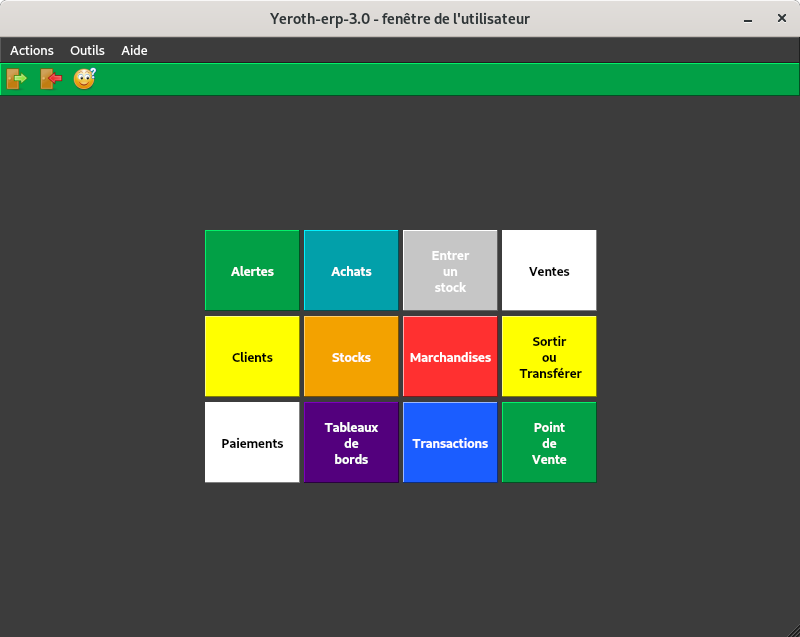
\includegraphics[scale=0.25]{images/yeroth-fenetre-manager.png}
\caption*{Manager's main window}
\end{center}
}
\end{tabular}
\end{table}

\vspace{0.7cm}

\begin{table}[!htbp]
\centering
\begin{tabular}{cccc}

\multicolumn{1}{c}{}			&
\yerotherp 						& 
\sageerp						&
\saperp		\\ \hline

\textbf{comprehensive training}		&
		\yerothvert{$3$ days}			&
		\yerothorange{$1$ month}			&						
		\yerothrouge{$2$ months}			\\ \hline

\textbf{software user interface}		&
		\yerothfacile					&
		\yerothdifficile				&						
		\yerothtresdifficile				\\  \hline
		
\textbf{usage language in software}			&
		\yerothvert{easy everyday English}	&
		\yerothorange{simple}					&						
		\yerothrouge{technical}					\\ \hline			
		
\textbf{financial accounting knowledge}	&
		\yerothvert{no}		&
		\yerothvert{no}		&						
		\yerothorange{useful}	\\ \hline		

\textbf{marketing knowledge}	&
		\yerothvert{no}			&
		\yerothorange{useful}	&						
		\yerothorange{useful}	\\ \hline
		
\textbf{internet}				&
		\yerothvert{no}			&
		\yerothrouge{mandatory}	&						
		\yerothrouge{mandatory}	\\		
\end{tabular}
\caption{Comparison between \yerotherp and other full featured ERP software--systems\\}
\label{tab:comparison-against-others-erp-software-systems}
\end{table}

\vspace{0.5cm}

Table~\ref{tab:comparison-against-others-erp-software-systems}
pictures the 'simplicity' and 'effectiveness' of \yerotherp, 
compared to other ERP software--systems such as
''\sageerp'', and ''\saperp''.\\


\vspace{1cm}

{\large \bf OPERATIONS}

\vspace{0.75em}

\begin{table}[!htbp]
\begin{tabular}{lll}

\begin{tcolorbox}[width=14.3em, boxrule=0.01em, colback=white]
\textbf{Point--of--Sale Hardware}
\vspace{-1em}
\hrule
\vspace{0.75em}
\begin{itemize}[]
	\item[\mycheckmark{yerothColorDarkgray}] Barcode scanner
	\item[\mycheckmark{yerothColorDarkgray}] Thermal printer, etc.\\
\end{itemize}
\begin{center}
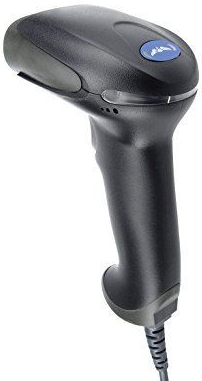
\includegraphics[scale=0.24]{images/xfox-fj-5-usb-plug-and-play-automatic-barcode-scanner.png}
\end{center}
\end{tcolorbox}

&

\begin{tcolorbox}[width=14.3em, boxrule=0.01em, colback=white]
\textbf{Database Management Systems}
\vspace{0.1em}
\hrule
\vspace{0.75em}
\begin{itemize}[]
	\item[\mycheckmark{yerothColorBlue}] \mysqlcolored\\
\end{itemize}
\begin{center}

\includegraphics[scale=0.14]{images/free-reuse-dbms-logo}
\end{center}
\end{tcolorbox}

&

\begin{tcolorbox}[width=14.3em, boxrule=0.01em, colback=white]
\textbf{Operating Systems}
\vspace{0.1em}
\hrule
\vspace{0.75em}
\begin{itemize}[]
	\item[\mycheckmark{yerothColorRed}] Debian--Linux\\	
\end{itemize}
\begin{center}

\includegraphics[scale=0.53]{images/free-reuse-stretch-logo}
\end{center}
\end{tcolorbox}

\end{tabular}
\end{table}


\end{document}

